% Тут используется класс, установленный на сервере Papeeria. На случай, если
% текст понадобится редактировать где-то в другом месте, рядом лежит файл matmex-diploma-custom.cls
% который в момент своего создания был идентичен классу, установленному на сервере.
% Для того, чтобы им воспользоваться, замените matmex-diploma на matmex-diploma-custom
% Если вы работаете исключительно в Papeeria то мы настоятельно рекомендуем пользоваться
% классом matmex-diploma, поскольку он будет автоматически обновляться по мере внесения корректив
%

% По умолчанию используется шрифт 14 размера. Если нужен 12-й шрифт, уберите опцию [14pt]
%\documentclass[14pt]{matmex-diploma}
\documentclass[14pt]{matmex-diploma-custom}

\usepackage{graphicx}
\usepackage{caption}
\usepackage{subcaption}

\newtheorem{theorem}{Theorem}

\begin{document}
% Год, город, название университета и факультета предопределены,
% но можно и поменять.
% Если англоязычная титульная страница не нужна, то ее можно просто удалить.
\filltitle{ru}{
    chair              = {Кафедра системного программирования},
    title              = {Синтаксический анализ данных, представленных в виде контекстно-свободной грамматики},
    % Здесь указывается тип работы. Возможные значения:
    %   coursework - Курсовая работа
    %   diploma - Диплом специалиста
    %   master - Диплом магистра
    %   bachelor - Диплом бакалавра
    type               = {diploma},
    position           = {студента},
    group              = 444,
    author             = {Ковалев Дмитрий Александрович},
    supervisorPosition = {к.\,ф.-м.\,н., *указать должность*},
    supervisor         = {Григорьев С.\,В.},
    reviewerPosition   = {программист *указать место работы*},
    reviewer           = {Авдюхин Д.\,А.},
    chairHeadPosition  = {д.\,ф.-м.\,н., профессор},
    chairHead          = {Терехов А.\,Н.},
%   university         = {Санкт-Петербургский Государственный Университет},
%   faculty            = {Математико-механический факультет},
%   city               = {Санкт-Петербург},
%   year               = {2013}
}
\filltitle{en}{
    chair              = {Chair of Software Engineering},
    title              = {Parsing of the data represented as \\ context free grammar},
    author             = {Dmitry Kovalev},
    supervisorPosition = {*position*},
    supervisor         = {Semyon Grigorev},
    reviewerPosition   = {Programmer at *company*},
    reviewer           = {Avdiukhin Dmitrii},
    chairHeadPosition  = {professor},
    chairHead          = {Christobal Junta},
}

\maketitle
\tableofcontents

\section*{Введение}

Контекстно-свободные грамматики, наряду с регулярными выражениями, активно используются для решения задач, связанных с разработкой формальных языков и синтаксических анализаторов. 
Одним из основных достоинств контекстно-свободных грамматик является возможность задания широкого класса языков при сохранении относительной компактности представления. 
Благодаря данному свойству, грамматики также представляют интерес в такой области информатики, как кодирование и сжатие данных. 
В частности, существует ряд алгоритмов, позволяющих производить сжатие текстовой информации, используя в качестве конечного \cite{sequitur} или промежуточного \cite{Arimura} представления контекстно-свободную грамматику (grammar-based compression). 

Стандартной процедурой при работе с текстовыми данными является поиск в них определенных шаблонов, которые могут быть заданы строкой или регулярным выражением. 
В настоящее время большие объемы информации, как правило, хранятся и передаются по сети в сжатом виде, поэтому актуальной задачей становится поиск шаблонов непосредственно в компактном контекстно-свободном представлении текста.
Такой подход позволяет избежать дополнительных затрат памяти на восстановление исходной формы данных и в некоторых случаях увеличивает скорость выполнения запроса.
Шаблон здесь может быть, как и при поиске в обычном тексте, строкой (compressed pattern matching), сжатой строкой (fully compressed pattern matching) или регулярным выражением.

Известны ситуации, в которых для задания шаблона необходимо использовать более выразительные средства. 
Примером может служить одна из задач биоинформатики --- поиск определенных подпоследовательностей в геноме организма. 
Так, для классификации и исследования образцов, полученных в результате процедуры секвенирования, в них могут искать гены, описывающие специфические рРНК. 
Структура таких генов, как правило, задается при помощи контекстно-свободной грамматики \cite{Anderson2013}. 
Для уменьшения объемов памяти, необходимых для хранения большого количества геномов, используются различные алгоритмы сжатия, в том числе основанные на получении контекстно-свободной структуры исходных последовательностей \cite{galle2011dna}.

Задача поиска КС-шаблонов при использовании КС-представления данных формулируется следующим образом: необходимо найти все строки, принадлежащие пересечению двух языков, один из которых задается грамматикой шаблона, а второй представляет собой язык всех подстрок исходного множества строк, описываемого грамматикой, полученной в результате сжатия данных.
Назовем такой поиск \textit{синтаксическим анализом данных, представленных в виде КС-грамматики}.
%В общем случае задача неразрешима, так как сводится к задаче о проверке пересечения двух языков, порождаемых произвольными КС-грамматиками, на пустоту \cite{harrison1978empt}.
Для постановки экспериментов в области биоинформатики необходимо точнее исследовать возможность проведения синтаксического анализа КС-представления и разработать прототип алгоритма, позволяющего решить данную задачу.

\section{Постановка задачи}
	Целью данной работы является разработка алгоритма синтаксического анализа данных, представленных в виде контекстно-свободной грамматики. Для ее достижения были поставлены следующие задачи.

\begin{itemize}
	\item Изучить существующие подходы к анализу данных, представленных в виде КС-грамматик.
	\item Определить ограничения, при которых синтаксический анализ такого представления является разрешимой задачей.
	\item Разработать алгоритм синтаксического анализа КС-представления данных с учетом поставленных ограничений и доказать его завершаемость.
	\item Реализовать предложенный алгоритм.
	\item Провести тестирование и апробацию.
\end{itemize}

\section{Обзор}

Пусть $G$ --- произвольная КС-грамматика, $M$ --- конечный автомат. Тогда задача проверки
\begin{itemize}
	\item включения языков ($L(M) \subseteq L(G)$) --- неразрешима
	\item пустоты пересечения ($L(M) \cap L(G) = \emptyset$) --- разрешима (т.к. в пересечении не более чем КС-язык) за полиномиальное время \cite{Hunt}
	\item регулярности языка $L(G)$ --- неразрешима \cite{Greibach1968}
\end{itemize} 

Если использовать представление регулярного языка $L(M)$ в виде КС-грамматики $G_r$, то задача проверки пустоты пересечения ($L(G_r) \, \cap \, L(G) = \emptyset$) становится немного интереснее: если $G_r$ 
\begin{itemize}
	\item нерекурсивная --- задача из PSPACE \cite{Nederhof} (точнее результата нет (я не нашел, по крайней мере))
	\item лево- или праволинейная --- ничего не известно (см. последний абзац заключения из \cite{Nederhof})
	\item принадлежит еще более широкому классу --- тем более ничего не известно
\end{itemize}

Еще немного про вложенную рекурсию и регулярность языка. Грамматика без вложенной рекурсии (NSE) порождает регулярный язык \cite{Chomsky} (обратное тоже верно, для регулярного языка можно построить NSE грамматику, т.к. праволинейная, например, --- частный случай NSE). Существует алгоритм, который позволяет проверять грамматику на наличие вложенной рекурсии за полином \cite{Anselmo}. Однако, грамматика с вложенной рекурсией тоже может порождать регулярный язык \cite{Andrei2004}, поэтому задача о проверке регулярности языка, порождаемого КС-грамматикой, остается неразрешимой. 

\section{Алгоритм}
	
Мы пытаемся решать следующую задачу: пусть $G_1 = (N, T, S, P)$ --- произвольная КС-грамматика, $G_2$ --- NSE КС-грамматика. Алгоритм принимает на вход два рекурсивных автомата, $M_1$ и $M_2$, построенных по грамматикам $G_1$ и $G_2$ соотвественно, при этом в автомате $M_2$ левые/правые рекурсивные вызовы заменены на циклы, как в обычном конечном автомате.

Результатом работы алгоритма являются тройки вида $(X, n_1, n_2)$, где $X \in N$, $n_1, n_2$ --- номера состояний автомата $M_2$. 
Для каждой из таких троек выполняется следующее утверждение: $\exists \, \omega \in T^*$ такая, что $X \rightarrow^* \omega$ в $G_1$ и $\omega \in L(M')$, где $M'$ --- рекурсивный автомат, полученный из $M_2$ путем замены начального и конечного состояния на $n_1$ и $n_2$ соответственно.
	
Получая такие результаты, мы, по сути, отвечаем на вопрос о проверке пустоты пересечения КС-языка и регулярного, представленных в необычных абстракциях. 
Для КС-языка мы используем рекурсивный автомат, а для регулярного --- нечто среднее между конечным автоматом и NSE грамматикой (это нечто все еще использует стек, но только для обработки нерекурсивных вызовов). 
Такое представление эквивалентно по выразительности NSE и, следовательно, FA (см. рис. \ref{circle:lang}). 
Но неизвестно, к какому классу сложности относится задача (и разрешима ли вообще) о проверке пустоты пересечения регулярного языка, представленного в данной форме, с КС-языком (см. рис. \ref{circle:intersec}).
	
\begin{theorem}{Завершаемость.}
	Алгоритм завершает работу за конечное число шагов для произвольных входных данных
\end{theorem}
	
\begin{theorem}{Корректность.}
	???
\end{theorem}

\begin{figure}[h!]
	\begin{subfigure}[t]{0.45\textwidth}
		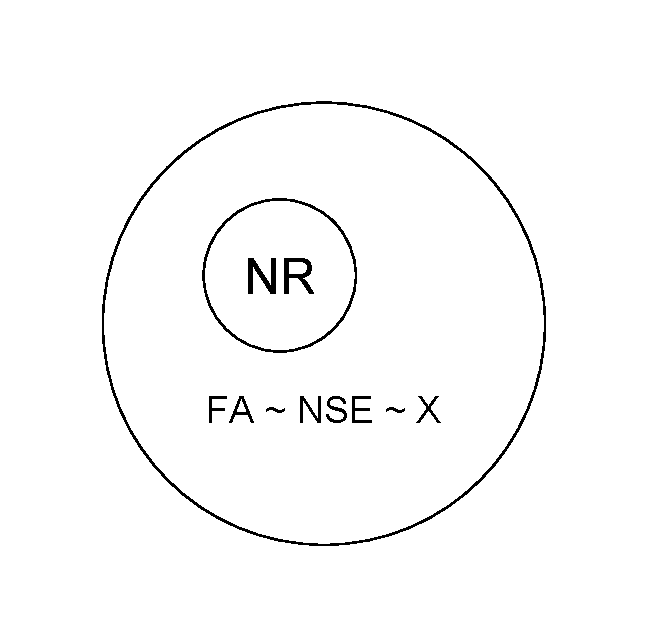
\includegraphics[width=\textwidth]{pictures/lang}
		\caption{Выразительность языка, задаваемого абстракцией}
		\label{circle:lang}
	\end{subfigure}
	~
	\begin{subfigure}[t]{0.45\textwidth}
		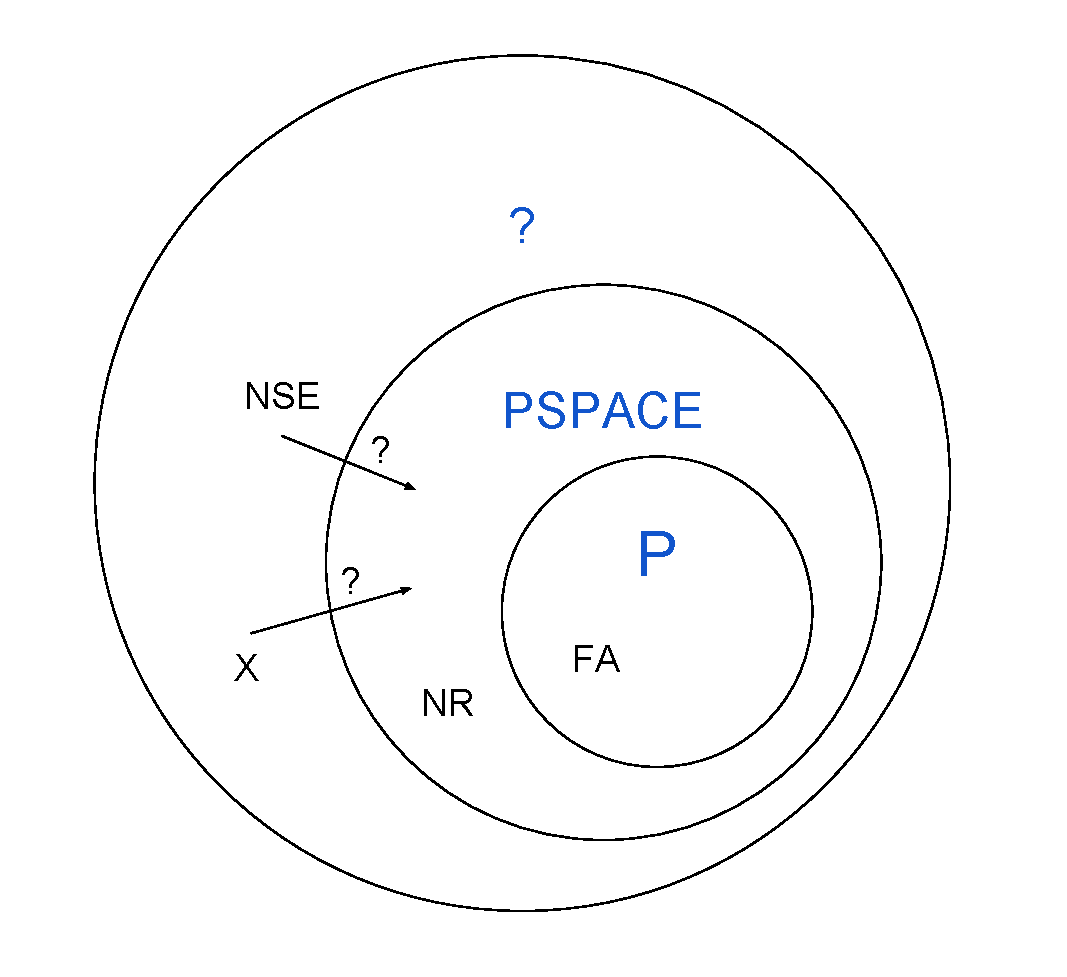
\includegraphics[width=\textwidth]{pictures/intersec_problem}
		\caption{Класс сложности для задачи о проверке пустоты пересечения с КС-языком}
		\label{circle:intersec}
	\end{subfigure}
	\caption{Красивые круги. Здесь NR --- нерекурсивная грамматика, FA --- конечный автомат, NSE --- грамматика без вложенной рекурсии, X --- наше представление}
	\label{circle}
\end{figure}

\setmonofont[Mapping=tex-text]{CMU Typewriter Text}
\bibliographystyle{ugost2008ls}
\bibliography{diploma.bib}
\end{document}